% =====================================================================
\section{Results}
\label{sec:results}
% =====================================================================

We first trace how the controller's initial advantage disappeared as its
comparators were corrected (RQ1, Section~\ref{sec:chain}), then measure
coordination itself (RQ2, Section~\ref{sec:coordination}), and then ask
what the corrected complete-policy comparison rests on: cluster size,
shedding, budgets, lag and the demand it was tuned for
(Sections~\ref{sec:remains}--\ref{sec:generalise}). Section~\ref{sec:level}
reports the final campaign, which removed every audited leak on both sides at
once; Section~\ref{sec:width} gives the mechanism, and Section~\ref{sec:live}
what ran on a real cluster. Throughout, $\Delta J$ is \jcac{} minus the comparator, so negative
values favour \jcac{}; tags such as JN-C1 name the registered test.

\subsection{How the initial advantage vanished}
\label{sec:chain}

\begin{figure}[t]
\centering
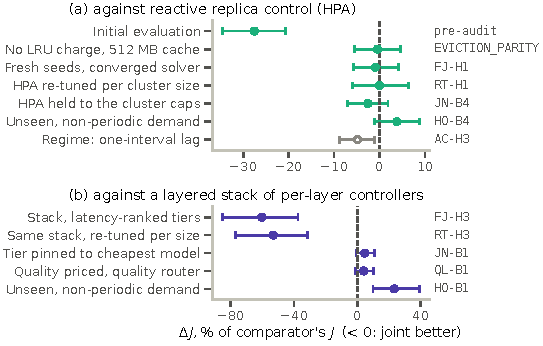
\includegraphics[width=\textwidth]{figures/fig_chain.pdf}
\caption{The joint controller's advantage disappears as its comparators
are corrected: \jcac{} minus comparator on $J$, per design point, as a
percentage of the comparator's $J$, with 95\% bootstrap intervals (negative:
\jcac{} better); each row keeps the corrections above it. The first two rows
of (a) are exploratory and did not share seeds; QL-B1 compares $J$ with
answer quality priced; the hollow row is a regime (replicas one interval
late), not a correction. The JN-B1 and HO-B1 stacks exceeded the cluster
caps; held to them, an exploratory re-run gives $-1.3\%$ and $+6.5\%$.}
\label{fig:chain}
\end{figure}

\emph{Against reactive replica control} (Fig.~\ref{fig:chain}(a)). The
pre-audit matrix put \jcac{} 27.5\% of HPA's $J$ ahead. Two comparator
defects produced that lead: only the comparators paid a $1.4581\times$
surcharge on inference cost (a model of LRU eviction that \jcac{}'s
cost-aware cache was assumed to avoid), and they ran a cache pinned at
128\,MB. Removing both erased it (EVICTION\_PARITY, $-0.4\%$). On fresh
shared seeds with the convergent solver the difference was $-0.0037$
$[-0.0234,+0.0166]$, a failed superiority test (FJ-H1). HPA's tuned target
lay on the edge of its grid; re-tuned per cluster size with an interior
optimum it tied again, $-0.0001$ $[-0.0239,+0.0257]$ (RT-H1), but the tie
hid a trade: \jcac{} spent 19.3\% less at 60.1\% higher mean violation, and
every SLO guard of that campaign failed. Held to the cluster caps that bind
\jcac{}, HPA still tied ($-0.0104$ $[-0.0290,+0.0076]$, JN-B4). \jcac{} beat
KEDA at its first fair setting ($-0.0305$, FJ-H2), tied it re-tuned
($-0.0309$ $[-0.0611,+0.0008]$, RT-H2) and beat it capped ($-0.0229$
$[-0.0438,-0.0022]$, JN-B5), a verdict that does not survive the
programme-wide correction.

\emph{Against a layered stack} (Fig.~\ref{fig:chain}(b)). The registered
layered stack lost by 60.4\% of its $J$ and, re-tuned per size, by 53.1\%
(FJ-H3, RT-H3), because its tier rule ranks tiers by latency and ignores
price: it reached the lowest violation of any arm at 3.4 times \jcac{}'s
spend (Table~\ref{tab:arms}). Pinned to the cheapest model, the same stack
tied \jcac{} ($+0.0178$ $[-0.0032,+0.0416]$, JN-B1), although it ran above
the cluster caps that bind \jcac{}; held to them, it still tied ($-0.0053$
$[-0.0201,+0.0092]$, exploratory). A cost-aware tier rule
lost by 0.3208 (JN-B2), and a quality-aware router tied when answer quality was priced (QL-B1).
The 53--60\% win measured one comparator's tier rule, not the value of
joint control.

Every defect we found in this chain had favoured the joint controller.
The corrections were applied one registered campaign at a time, and each
earlier record stands unedited beside its successor.

\subsection{What coordination is worth}
\label{sec:coordination}

\begin{table}[t]
\caption{Coordination in every registered setting where joint and
decoupled search ran on the same units: $\Delta J$ = joint minus decoupled
(negative: joint better), 95\% bootstrap CI, and the gain as a percentage
of the decoupled arm's $J$. EQ: CI inside $\pm0.025$. The width rows score
the 48 AI-carrying design points on the rate-limited lattice.}
\label{tab:coord}
\centering\footnotesize\setlength{\tabcolsep}{2.5pt}
\begin{tabular}{@{}l l r c r l@{}}
\toprule
Setting & Test & $\Delta J$ & 95\% CI & Gain & Reading \\
\midrule
Main matrix & JN-C1 & $-0.0066$ & $[-0.0121,-0.0022]$ & $+1.6\%$ & PASS, EQ \\
Cache curve fitted to LMSYS & CS-EQ & $-0.0064$ & $[-0.0110,-0.0029]$ & $+1.4\%$ & EQ \\
Published cache curve (rerun) & CS-EQ & $-0.0053$ & $[-0.0102,-0.0015]$ & $+1.3\%$ & EQ \\
High cache curve & CS-EQ & $-0.0042$ & $[-0.0085,-0.0009]$ & $+1.1\%$ & EQ \\
Answer quality priced ($J_q$) & QL-C1 & $+0.0012$ & $[-0.0016,+0.0043]$ & $-0.3\%$ & tie, EQ \\
Real BurstGPT windows & TA-EQ & $-0.0025$ & $[-0.0037,-0.0013]$ & $+0.6\%$ & EQ \\
Unseen, non-periodic demand & HO-C1 & $+0.0045$ & $[+0.0020,+0.0073]$ & $-1.4\%$ & worse, EQ \\
Live-fitted plant & RV-L-EQ & $-0.0017$ & $[-0.0028,-0.0008]$ & $+1.3\%$ & EQ \\
Width: published plant & WD-H4 & $-0.0044$ & $[-0.0088,-0.0006]$ & $+0.7\%$ & EQ \\
Width: coupled plant & WD-H4 & $-0.0092$ & $[-0.0181,-0.0019]$ & $+0.9\%$ & EQ \\
Width: live-fitted plant & WD-H4 & $-0.0033$ & $[-0.0048,-0.0019]$ & $+1.3\%$ & EQ \\
\bottomrule
\end{tabular}
\end{table}

With objective, forecast, budget filter, caps and lattice held fixed,
joint search lowered $J$ by $0.0066$ $[0.0022,0.0121]$ relative to
decoupled search, 1.6\% of the decoupled arm's $J$, and by $0.0009$
relative to knob-wise search (JN-C1, JN-C2; Table~\ref{tab:coord}). Both
reductions passed their directional tests (JN-C1 survives the
programme-wide Benjamini--Yekutieli correction but not Holm), and both lie
inside the equivalence margin. The decoupled arm spent 1.5\% less and violated
slightly more; coordination bought a little attainment, not savings.

Three qualifications bound this reading. First, the average is diluted: on
the 24 CRUD-only design points the two searches scored identically, as they
must when only the replica knob acts. On the 36 AI-carrying points the gain
was $0.0109$ $[0.0039,0.0198]$, and on the 12 small-cluster AI points
$0.0282$ $[0.0109,0.0503]$ (exploratory), an interval that reaches past the
margin. Second, the margin of $\pm0.025$ was set from the detectable
difference of the comparator contrasts; the joint--decoupled contrast is
far less noisy (its own detectable difference is about $0.007$), so
``inside the margin'' is a weak statement for it, and the interval itself,
0.5--3.0\% of $J$ overall, is the informative reading. Third, the
directional part rests on an unmeasured constant: with a monotone agent
latency ladder (small 0.94\,s, mid 2.5\,s, large 3.5\,s) and nothing else
changed, an exploratory re-run of one replication found no coordination
gain at all ($+0.0017$ $[-0.0020,+0.0061]$).

The result does not hinge on the synthetic cache curve or on the
objective. Under the cache curve fitted to real LMSYS prompts and under a
high one, $0.95\,c/(c+128)$, the reduction was 1.4\% and 1.1\% of $J$
(CS). With twice the answer-quality loss of Table~\ref{tab:tiers} added to
$J$, measured GPU prices and no budget filter, the difference was
$+0.0012$ (QL-C1), and on unseen demand decoupled search was the better of
the two, inside the margin (HO-C1). In all eleven registered settings the
difference stayed inside the registered margin.

\subsection{The complete policy after the corrections}
\label{sec:remains}

\begin{table}[t]
\caption{Mean outcome per arm in JOINTNESS (60 design points $\times$ 5
replications, shared seeds). Cost: simulated dollars per run. Viol.: mean
SLO violation. Excess: uncapped overshoot. Shed: tenant-steps with AI on
tier ``none''. Over.: tenant-steps over the tenant's budget (\jcac{} filters
on projected, not realised, cost).}
\label{tab:arms}
\centering\tablefont
% generated by make_assets.py -- do not edit
\begin{tabular}{@{}l r r r r r r@{}}
\toprule
Arm & $J$ & Cost & Viol. & Excess & Shed & Over. \\
 & & (\$) & & & (\%) & (\%) \\
\midrule
\jcac{}, joint search & 0.3991 & 2.36 & 0.068 & 0.207 & 7.2 & 0.9 \\
\jcac{}, decoupled search & 0.4057 & 2.33 & 0.072 & 0.209 & 7.7 & 0.8 \\
\jcac{}, knob-wise search & 0.4000 & 2.36 & 0.068 & 0.207 & 7.3 & 0.8 \\
\jcac{}, plans on violation & 0.4038 & 2.06 & 0.084 & 0.465 & 12.5 & 0.9 \\
\jcac{}, never sheds & 0.4668 & 2.81 & 0.075 & 0.533 & 0.0 & 4.5 \\
\midrule
Layered, cheapest tier & 0.3814 & 2.70 & 0.045 & 0.130 & 0.0 & 3.1 \\
Layered, cost-aware tier & 0.7199 & 4.35 & 0.113 & 0.630 & 0.0 & 7.3 \\
Layered, registered rule & 0.8631 & 7.97 & 0.012 & 0.029 & 0.0 & 10.4 \\
\midrule
Static equal share & 0.4226 & 2.91 & 0.052 & 0.177 & 0.0 & 3.5 \\
HPA, re-tuned & 0.4006 & 2.92 & 0.043 & 0.104 & 0.0 & 3.8 \\
HPA, re-tuned, capped & 0.4095 & 2.77 & 0.053 & 0.187 & 0.0 & 3.6 \\
KEDA, re-tuned, capped & 0.4220 & 2.93 & 0.051 & 0.172 & 0.0 & 3.8 \\
\bottomrule
\end{tabular}

\end{table}

\begin{table}[t]
\caption{What survives the corrections: \jcac{} minus comparator on $J$
(mean paired difference over design points, 95\% bootstrap CI; negative:
\jcac{} better). B: better; T: tie; W: worse; EQ: inside the $\pm0.025$
margin. The cheapest-tier stack was not held to the cluster caps (see
Section~\ref{sec:comparators}).}
\label{tab:post}
\centering\tablefont
% generated by make_assets.py -- do not edit
\begin{tabular}{@{}l l r c l@{}}
\toprule
Comparator & Test & $\Delta J$ & 95\% CI & \\
\midrule
\multicolumn{5}{@{}l}{\textit{Instant actuation} (60 design points)} \\
\quad Decoupled search & \texttt{JN-C1} & $-0.0066$ & $[-0.0121,-0.0022]$ & B, EQ \\
\quad Layered, cheapest tier & \texttt{JN-B1} & $+0.0178$ & $[-0.0032,+0.0416]$ & T \\
\quad Static equal share & \texttt{JN-B3} & $-0.0235$ & $[-0.0422,-0.0050]$ & B \\
\quad HPA, re-tuned, capped & \texttt{JN-B4} & $-0.0104$ & $[-0.0290,+0.0076]$ & T \\
\quad KEDA, re-tuned, capped & \texttt{JN-B5} & $-0.0229$ & $[-0.0438,-0.0022]$ & B \\
\midrule
\multicolumn{5}{@{}l}{\textit{Replicas one interval late} (60 design points)} \\
\quad Layered, cheapest tier & \texttt{AC-H1} & $+0.0069$ & $[-0.0135,+0.0300]$ & T \\
\quad Static equal share & \texttt{AC-H2} & $-0.0227$ & $[-0.0416,-0.0040]$ & B \\
\quad HPA, re-tuned, capped & \texttt{AC-H3} & $-0.0204$ & $[-0.0371,-0.0045]$ & B \\
\quad KEDA, re-tuned, capped & \texttt{AC-H4} & $-0.0279$ & $[-0.0474,-0.0089]$ & B \\
\midrule
\multicolumn{5}{@{}l}{\textit{Unseen, non-periodic demand} (24 design points)} \\
\quad Decoupled search & \texttt{HO-C1} & $+0.0045$ & $[+0.0020,+0.0073]$ & W, EQ \\
\quad Layered, cheapest tier & \texttt{HO-B1} & $+0.0629$ & $[+0.0268,+0.1065]$ & W \\
\quad Static equal share & \texttt{HO-B3} & $-0.0109$ & $[-0.0323,+0.0112]$ & T \\
\quad HPA, re-tuned, capped & \texttt{HO-B4} & $+0.0122$ & $[-0.0035,+0.0284]$ & T \\
\quad KEDA, re-tuned, capped & \texttt{HO-B5} & $-0.0151$ & $[-0.0377,+0.0073]$ & T \\
\bottomrule
\end{tabular}

\end{table}

\begin{figure}[t]
\centering
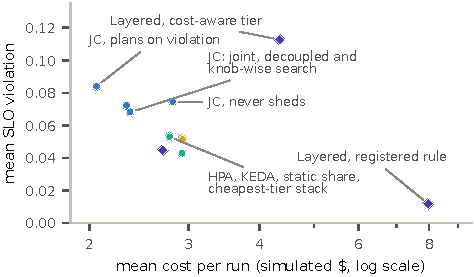
\includegraphics[width=0.62\textwidth]{figures/fig_tradeoff.pdf}
\caption{\jcac{} is the cheapest arm and among the most violating: mean
cost against mean SLO violation for every arm of Table~\ref{tab:arms}
(JOINTNESS). HPA, KEDA, the static share and the cheapest-tier stack
cluster at lower violation and 14--24\% higher cost; the never-shedding
variant of \jcac{} loses its cost advantage.}
\label{fig:tradeoff}
\end{figure}

With the defects removed, the complete-policy comparison is close
(Tables~\ref{tab:arms} and~\ref{tab:post}). \jcac{} tied capped HPA and the
cheapest-tier stack, and beat capped KEDA and the static share by
$0.0229$ and $0.0235$ in $J$, about 5.5\% (JN-B5, JN-B3). Its SLO guard
failed against all four: \jcac{}'s mean violation was 0.068, against
0.043--0.053 for every HPA, KEDA, static and cheapest-tier arm, which cost
14--24\% more (Fig.~\ref{fig:tradeoff}). Neither of the two wins survives
the programme-wide Holm correction.

\begin{figure}[t]
\centering
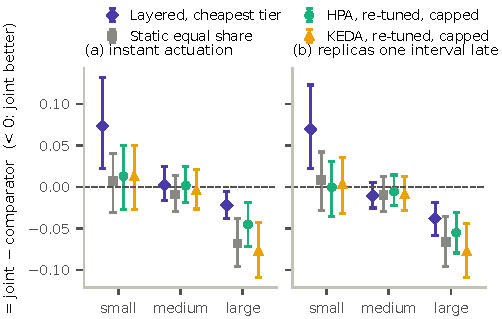
\includegraphics[width=0.62\textwidth]{figures/fig_sizes.pdf}
\caption{Every win of \jcac{} comes from the large cluster: \jcac{} minus
comparator on $J$ per cluster size, 20 design points each, 95\% bootstrap
intervals, (a) with instant actuation (JOINTNESS) and (b) with replicas
one interval late (ACTUATION). On the small cluster the cheapest-tier stack
is better in both regimes, but it ran twice that cluster's replica cap; held
to the caps it ties (exploratory, not plotted).}
\label{fig:sizes}
\end{figure}

The wins are not spread across the matrix (Fig.~\ref{fig:sizes}).
\jcac{} beat every comparator on the large cluster, by $0.0220$ to $0.0771$
in $J$ against the four competitive ones; it tied every one on the medium
cluster; and on the small cluster the cheapest-tier stack beat it by
$0.0732$ $[0.0227,0.1314]$, but that stack ran twice the small cluster's
replica cap there, and held to the caps it tied \jcac{} ($+0.0066$,
exploratory). By workload,
the wins came with the CRUD classes, where only the replica knob acts and
\jcac{} was better than every comparator but the cost-aware stack on all 12
steady-CRUD design points: on the 24 CRUD points it beat capped KEDA and the
static share by about 0.05 in $J$, which is replica sizing against
comparators whose single tuned target over-provisions CRUD
(Section~\ref{sec:comparators}). On the 36 design points that carry AI
traffic, where the cache and tier knobs act, \jcac{} tied capped HPA
($-0.0043$ $[-0.0341,+0.0245]$), capped KEDA ($-0.0053$) and the static
share ($-0.0056$), and lost to the uncapped cheapest-tier stack ($+0.0446$
$[+0.0124,+0.0809]$); on the agentic class it was worse than every
comparator except the cost-aware stack. Nor did it use its tier knob much:
it chose the large tier on no tenant-step and the mid tier on 1.7\%, so in
practice its tier decision was ``small or shed''. The controller built to
coordinate the AI knobs gained nothing on the workloads those knobs serve.

\subsection{Where the savings come from: shedding}
\label{sec:shed}

\begin{table}[t]
\caption{Total cost and cost per request actually served. Shed: share of
requests answered by no model. Unit: the ratio averaged over design points
(main matrix) or windows (BurstGPT); pooled: taken over all requests of all
runs (exploratory). Counts come from request counters added to the
simulator without changing any registered metric (SA: 27{,}720 registered
values replayed bit-identically).}
\label{tab:served}
\centering\footnotesize\setlength{\tabcolsep}{2.5pt}
\begin{tabular}{@{}l r r r r r@{}}
\toprule
 & Cost & Shed (\%) & Shed (\%) & \$/1{,}000 served & \$/1{,}000 served \\
Arm & (\$/run) & unit & pooled & unit & pooled \\
\midrule
\multicolumn{6}{@{}l}{\textit{Main matrix (JN runs, 180{,}773 requests per run)}} \\
\quad \jcac{}, joint search & 2.363 & 5.7 & 2.1 & 0.0340 & 0.01335 \\
\quad \jcac{}, decoupled search & 2.328 & 6.0 & 2.2 & 0.0336 & 0.01317 \\
\quad \jcac{}, never sheds & 2.809 & 0.0 & 0.0 & 0.0367 & 0.01554 \\
\quad HPA, re-tuned, capped & 2.775 & 0.0 & 0.0 & 0.0338 & 0.01535 \\
\quad KEDA, re-tuned, capped & 2.926 & 0.0 & 0.0 & 0.0349 & 0.01619 \\
\quad Layered, cheapest tier & 2.698 & 0.0 & 0.0 & 0.0331 & 0.01493 \\
\quad Static equal share & 2.910 & 0.0 & 0.0 & 0.0348 & 0.01610 \\
\midrule
\multicolumn{6}{@{}l}{\textit{Real BurstGPT windows (TA runs, 804{,}710 requests per run)}} \\
\quad \jcac{}, joint search & 34.70 & 14.7 & 42.8 & 0.4687 & 0.07545 \\
\quad \jcac{}, decoupled search & 34.24 & 15.0 & 43.4 & 0.4689 & 0.07523 \\
\quad \jcac{}, never sheds & 79.00 & 0.0 & 0.0 & 0.4783 & 0.09817 \\
\quad HPA, re-tuned, capped & 69.52 & 0.0 & 0.0 & 0.2950 & 0.08640 \\
\quad KEDA, re-tuned, capped & 69.94 & 0.0 & 0.0 & 0.3001 & 0.08691 \\
\quad Layered, cheapest tier & 68.06 & 0.0 & 0.0 & 0.2890 & 0.08457 \\
\quad Static equal share & 76.17 & 0.0 & 0.0 & 1.2468 & 0.09465 \\
\bottomrule
\end{tabular}
\end{table}

\jcac{} shed AI traffic on 7.2\% of tenant-steps. Request counters, added to
the simulator as a registered re-run that left every registered metric
bit-identical (SA), show what that means: on the mean design point it left
10.1\% of AI requests (5.7\% of all requests) unanswered by any model, and
35.3\% of the agentic class's AI requests (Table~\ref{tab:served}). On the
BurstGPT windows it left 14.7\% unserved on the mean window and 42.8\% of
all requests pooled, because it sheds when demand, and so spend, peaks. The
decoupled and knob-wise arms shed as often (7.7\% and 7.3\% of
tenant-steps), so the savings come from shedding, not from coordination.

Shedding is where the cost advantage lives. Forbidden to shed, \jcac{} cost
19\% more than with shedding, slightly more than capped HPA; its $J$ rose by
$0.0677$ $[0.0432,0.0945]$, and it lost to capped HPA by $0.0573$
$[0.0225,0.0938]$ (JOINTNESS) and, on the BurstGPT windows, by $0.2229$.
That registered variant is handicapped, however: when no affordable
candidate exists, its fallback cuts two replicas and a cache level while
still serving over budget, so it misses more and pays more. With a fallback
that holds its configuration instead, an exploratory re-run of the AI
design points (one replication) improved its $J$ by 0.096 at 2.7\% lower
cost, which would put it close to capped HPA overall. The cost increase of
forbidding shedding (16--19\%) survives that correction; the loss to capped
HPA may not.

Billing each shed request at the cheapest tier's price, as if it had been
served there, removes every dollar advantage \jcac{} has and, in $J$, turns
the tie with capped HPA into a loss ($+0.0295$ $[0.0045,0.0562]$) and the
wins over capped KEDA and the static share into ties (exploratory
re-scoring of the registered runs). Per AI request actually served,
\jcac{} paid the most of the main arms (\$0.110 per 1{,}000 against
\$0.103 for the cheapest-tier stack and \$0.106 for capped HPA; 7--9\% more
on the small cluster), because it holds less cache and buys the mid tier for
some agent traffic (exploratory, one replication). Over all requests,
whether \jcac{} is cheaper per request served depends on how the ratio is
aggregated (Table~\ref{tab:served}): per design point or window it is not
(dearer than the cheapest-tier stack by 2.7\% on the matrix and 62\% on the
BurstGPT windows); pooled over requests it is about 11\% cheaper, because
cheap CRUD requests dominate the pool and it drops the most traffic where
traffic is heaviest. We claim no per-request saving.

Not every shed is the objective's choice (exploratory analysis of one
replication; the registered SA record counts sheds but not their cause). Of
\jcac{}'s shed decisions on
the AI design points, 58\% were forced: no candidate fit the budget. The
other 42\% were voluntary (an affordable candidate existed), including every
shed of a premium tenant. The budgets themselves set the scale of the
forced part: on the BurstGPT windows a \$5 hourly budget pays for at most
about 19 chat requests per second even on the small tier with a full cache,
while heavy windows average 11--17 and peak at 50 per tenant, so much of the
42.8\% pooled shed reflects the budgets we chose, not only the controller.

$J$ is what makes this pay. As derived in Section~\ref{sec:objective}, $J$
values an AI outage at no more than $2q_{\mathrm{AI}}$ per tenant-step,
less than the model spend of many intervals. Adding $\kappa s$ to $J$, with
$s$ the share of tenant-steps an arm sheds, erases \jcac{}'s wins over
capped KEDA and the static share at $\kappa\approx0.32$ (95\% intervals
within $[0.02,0.79]$) and its point advantage over capped HPA at
$\kappa\approx0.14$ (exploratory, RV); for scale, \jcac{}'s $J$ is 0.40. On the
live-fitted plant, where no comparator ever violated an SLO, \jcac{} still
shed on 14.2\% of tenant-steps, cost more than the cheapest-tier stack
(\$1.16 against \$1.02 per run) and lost to it by $0.0268$ in $J$ (RV-L3):
there, the (uncapped) stack serving every request on the cheapest model
dominated the joint controller on cost, violation and fairness at once.

\subsection{Budgets and actuation lag}
\label{sec:budget}

Only \jcac{} filters its candidates by the tenant's budget, which can only
hurt it on $J$ (which ignores budgets), so BM re-ran the comparators under
the same filter. Capped HPA and KEDA then lost to \jcac{} by $0.0316$
$[0.0154,0.0495]$ and $0.0416$ $[0.0242,0.0598]$ on the main matrix
(BM-H1, BM-H2) and by about 0.17 on the BurstGPT windows; the
budget-filtered cheapest-tier stack still tied ($-0.0011$
$[-0.0221,+0.0212]$, BM-H3). These wins must be read for what the filter
did. Because the comparators' cache and tier rules stayed their own, the
filter could only trim replicas; it lowered their spend by about 1\% and
left them over budget on 2.2--3.2\% of tenant-steps, while raising their
violation by about 0.009 (on the windows, from 0.017 to 0.074). BM therefore
shows that trimming replicas to meet a budget does not work when model
spend dominates, as an earlier campaign had predicted
(BUDGET\_PARITY), not that \jcac{} beats a budget-compliant autoscaler.
No budget-compliant comparator that serves every request exists in this
plant; the fair comparator, a per-layer stack whose gateway refuses AI
calls once a tenant's budget is spent, is the gated stack of the final
campaign (Section~\ref{sec:level}).

Actuation lag is the one regime in which \jcac{} beat the reactive rules
with its SLO guard intact. With replica changes taking effect one interval
late and enlarged caches half-warm, \jcac{} beat capped HPA by 4.8\%
($-0.0204$ $[-0.0371,-0.0045]$, AC-H3) and capped KEDA by 6.5\%
($-0.0279$, AC-H4), and both guards passed: a planner with a horizon
anticipates what a reactive rule can only follow. It still tied the
cheapest-tier stack (AC-H1), tier switches never lagged, and the plant had
no request backlog. Both verdicts survive the programme-wide
Benjamini--Yekutieli correction but not Holm.

\subsection{Generalisation}
\label{sec:generalise}

Every positive result above was obtained on the periodic workloads that
the comparators were tuned on. On two held-out Markov-modulated workloads,
registered before any arm ran on them, \jcac{} beat no comparator, and the
cheapest-tier stack beat it by $0.0629$ $[0.0268,0.1065]$, 23.3\% of the
stack's $J$, on every cluster size, the large one included (HO-B1;
Table~\ref{tab:post}, last block). Every SLO guard failed: the stack held
violation at 0.004 against \jcac{}'s 0.056, while \jcac{} shed on 11.3\% of
tenant-steps. Part of that margin was the stack's excess hardware: held to
the cluster caps (exploratory), it still beat \jcac{}, by $0.0202$
$[0.0039,0.0361]$ or 6.5\% of its $J$.

On the 96 real BurstGPT windows, \jcac{} beat only the static share
($-0.0913$ $[-0.1751,-0.0290]$, TA-H4), at an SLO excess of 0.34 against
0.02. It did not beat capped HPA ($-0.0530$ $[-0.1376,+0.0095]$, better in
31\% of windows), capped KEDA, or the uncapped cheapest-tier stack
($-0.0132$ $[-0.0611,+0.0239]$, better in 23\% of windows). On a plant re-fitted to
the deployed gateway's measurements, a planner that kept believing the
published plant lost to the registered layered stack by $0.1052$
(SM-H2[live]), and \jcac{} planning on the fitted plant trailed the
uncapped cheapest-tier stack by $0.0268$ (RV-L3). None of the joint controller's
advantages over a tuned, cheapest-model per-layer stack holds outside the
setting it was designed in.

\subsection{At a level field: the final campaign}
\label{sec:level}

\begin{table}[t]
\caption{LEVEL, the final campaign (8{,}832 runs, all valid, fresh seeds):
the corrected joint controller minus each comparator on $J_L$ (the objective
with every refused request charged the small tier's price), mean paired
difference over design points or windows and 95\% bootstrap CI (negative:
\jcac{} better). One Holm family of eleven; below the rule, coordination
(joint minus decoupled search) against the registered $\pm0.01$ margin.}
\label{tab:level}
\centering\scriptsize\setlength{\tabcolsep}{2.5pt}
% generated by make_tables.py -- do not edit
\begin{tabular}{@{}l l l r c l@{}}
\toprule
Test & Substrate & Comparator & $\Delta J_L$ & 95\% CI & Verdict \\
\midrule
\texttt{LV-B1} & main & Cheapest-tier stack, budget-gated & $+0.0038$ & $[-0.0130,+0.0207]$ & FAIL \\
\texttt{LV-B2} & main & HPA, capped & $+0.0208$ & $[-0.0026,+0.0441]$ & FAIL \\
\texttt{LV-B3} & main & KEDA, capped & $+0.0088$ & $[-0.0174,+0.0350]$ & FAIL \\
\texttt{LV-B4} & main & Cheapest-tier stack, capped & $+0.0282$ & $[+0.0070,+0.0496]$ & FAIL \\
\texttt{LV-B5} & main & Static equal share & $+0.0081$ & $[-0.0164,+0.0324]$ & FAIL \\
\texttt{LV-P1} & main & JC, published & $-0.0095$ & $[-0.0234,+0.0040]$ & FAIL \\
\texttt{LV-R1} & mono & Cheapest-tier stack, budget-gated & $+0.0046$ & $[-0.0121,+0.0207]$ & FAIL \\
\texttt{LV-L1} & lag & Cheapest-tier stack, budget-gated & $+0.0335$ & $[+0.0108,+0.0560]$ & FAIL \\
\texttt{LV-L2} & lag & HPA, capped & $+0.0518$ & $[+0.0245,+0.0789]$ & FAIL \\
\texttt{LV-O1} & held-out & Cheapest-tier stack, budget-gated & $+0.1230$ & $[+0.0982,+0.1484]$ & FAIL \\
\texttt{LV-T1} & BurstGPT & Cheapest-tier stack, budget-gated & $-0.0152$ & $[-0.0186,-0.0118]$ & PASS \\
\midrule
\texttt{LV-C[LV]} & main & decoupled search & $-0.0119$ & $[-0.0173,-0.0071]$ & not EQ at $\pm0.01$ \\
\texttt{LV-C[MO]} & mono & decoupled search & $-0.0120$ & $[-0.0181,-0.0065]$ & not EQ at $\pm0.01$ \\
\texttt{LV-C[LG]} & lag & decoupled search & $-0.0095$ & $[-0.0143,-0.0053]$ & not EQ at $\pm0.01$ \\
\texttt{LV-C[HO]} & held-out & decoupled search & $-0.0212$ & $[-0.0300,-0.0127]$ & not EQ at $\pm0.01$ \\
\texttt{LV-C[TR]} & BurstGPT & decoupled search & $-0.0070$ & $[-0.0097,-0.0046]$ & EQ at $\pm0.01$ \\
\bottomrule
\end{tabular}

\end{table}

\begin{table}[t]
\caption{Mean outcome per arm in LEVEL's main matrix (60 design points
$\times$ 5 replications). Shed: share of requests refused; Over.:
tenant-steps over budget. Every arm obeys the cluster caps.}
\label{tab:levelarms}
\centering\footnotesize\setlength{\tabcolsep}{4pt}
% generated by make_tables.py -- do not edit
\begin{tabular}{@{}l r r r r r r@{}}
\toprule
Arm & $J_L$ & $J$ & Cost & Viol. & Shed & Over. \\
 & & & (\$) & & (\%) & (\%) \\
\midrule
JC, level (treatment) & 0.4278 & 0.4076 & 2.31 & 0.074 & 3.2 & 0.7 \\
JC, level, decoupled search & 0.4398 & 0.4148 & 2.28 & 0.079 & 3.9 & 0.7 \\
JC, published & 0.4374 & 0.3972 & 2.35 & 0.068 & 5.8 & 0.8 \\
\midrule
Cheapest-tier stack, budget-gated & 0.4240 & 0.4069 & 2.51 & 0.066 & 2.3 & 0.7 \\
Cheapest-tier stack, capped & 0.3997 & 0.3997 & 2.67 & 0.054 & 0.0 & 3.3 \\
HPA, capped & 0.4070 & 0.4070 & 2.77 & 0.053 & 0.0 & 3.6 \\
KEDA, capped & 0.4191 & 0.4191 & 2.93 & 0.051 & 0.0 & 3.8 \\
Static equal share & 0.4197 & 0.4197 & 2.91 & 0.052 & 0.0 & 3.6 \\
\bottomrule
\end{tabular}

\end{table}

The twelfth campaign removed the audited leaks on both sides at once
(Section~\ref{sec:levelmethod}) and asked RQ1 and RQ2 again on fresh seeds.
All 8{,}832 runs were valid; of eleven registered tests, one passed
(Table~\ref{tab:level}). We had predicted three passes, and all three failed;
the one test that passed was predicted to fail.

On the main matrix the corrected controller beat no comparator. It tied the
budget-gated stack ($+0.0038$ $[-0.0130,+0.0207]$), capped HPA, capped KEDA
and the static share, and the capped cheapest-tier stack without a gate was
better than it ($+0.0282$ $[+0.0070,+0.0496]$; Table~\ref{tab:levelarms}). The
fixes did not make it better than the published controller under $J_L$
($-0.0095$ $[-0.0234,+0.0040]$): pricing the outage cut its refused share from
5.8\% to 3.2\% of requests, but its violation rose from 0.068 to 0.074. The
monotone agent row changed nothing (LV-R1). Under one-interval actuation lag
the corrected controller lost to the gated stack ($+0.0335$) and to capped HPA
($+0.0518$), the reverse of ACTUATION. The arms explain why: under lag its $J_L$
rose by 0.043, the published controller's by 0.001. The published switching
penalty ratchets replicas upward (Section~\ref{sec:objective}); under instant
actuation that is a defect, but under lag it is a hedge, and the corrected
penalty, which lets replicas fall and rise again, pays for every replica that
arrives late. The variant was chosen under instant actuation, where that cost
is invisible. On the held-out workloads the gated stack beat it by $0.1230$
$[0.0982,0.1484]$.

The one registered win came on the real BurstGPT windows, where the budgets
bind hardest. Among the arms that keep the budget, the corrected controller
beat the budget-gated stack by $0.0152$ $[0.0118,0.0186]$, 2.7\% of the stack's
$J_L$, in 91\% of windows, at 13\% lower cost and the same refused share (14.4\%
of requests): budget-aware joint planning beat a reactive gate there. The
comparators that ignore the budget (capped HPA, capped KEDA and the ungated
stack), which spent more than twice as much and served every request, scored
better than both ($J_L$ 0.439--0.441 against 0.552). Which of the two is
preferable depends on whether a budget is a hard constraint; $J_L$ treats it
as a soft one.

Coordination grew once outages were priced (Table~\ref{tab:level}, lower
block): joint search beat decoupled search by 1.3--4.5\% of $J_L$, with every
interval below zero. Only on the BurstGPT windows did the difference fall
inside the registered $\pm0.01$ margin, and on the held-out workloads (4.5\%) it
exceeded even $\pm0.025$. The mechanism of Section~\ref{sec:width} bounds
coordination; it does not make it zero. When a refused request costs money,
the planner has more to trade between cache and tier, and the gain grows by
about two-thirds over JOINTNESS. It still bought no win against a level
per-layer stack.

\subsection{Why coordination buys little}
\label{sec:width}

For a move $\delta=(\delta_r,\delta_c,\delta_\tau)$ of one tenant, the
second-order change in $\Phi$ is
$\sum_k g_k\delta_k+\frac12\sum_{k,l}H_{kl}\delta_k\delta_l$. Decoupled
search sees every term except the cross terms ($k\neq l$), so it recovers the
joint move unless a cross term reverses a per-knob choice. First-order gains
grow with $|\delta|$ and cross terms with $|\delta|^2$, so small steps make
reversals rare. Near a resting optimum the gradient vanishes and
separability needs small cross terms instead, which is what Bristol's
relative gain array tests~\cite{bristol1966}. In this plant, cache and tier
always interact through the price of a miss, and the replica knob interacts
with the others only where AI work loads the replicas. The argument is a
heuristic (the tier is categorical), but it makes two predictions:
coordination should grow with the step size, and only on plants where the
layers share capacity.

\begin{figure}[t]
\centering
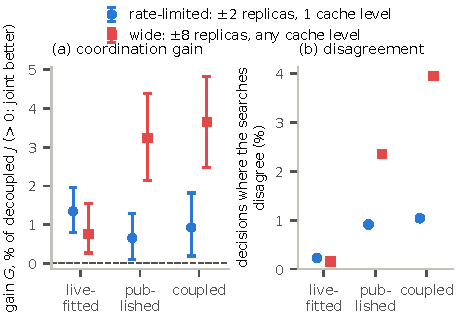
\includegraphics[width=0.62\textwidth]{figures/fig_width.pdf}
\caption{Coordination grows with step width, and only on plants where AI
work loads the replicas. (a) Gain $G=J(\text{decoupled})-J(\text{joint})$
as a percentage of the decoupled arm's $J$, with 95\% bootstrap intervals.
(b) Share of best responses in which decoupled search would choose
differently. 48 AI-carrying design points $\times$ 5 replications per
plant.}
\label{fig:width}
\end{figure}

\begin{table}[t]
\caption{The width experiment: coordination gain $G$ on the rate-limited
($n$) and wide ($w$) lattices, their difference-in-differences (DiD), and
the joint controller's own $J$ on the rate-limited minus the wide lattice
(negative: rate-limited better).}
\label{tab:width}
\centering\tablefont
% generated by make_assets.py -- do not edit
\begin{tabular}{@{}lrrcr@{}}
\toprule
Plant & $G_n$ & $G_w$ & DiD [95\% CI] & $J_n-J_w$ \\
\midrule
Live-fitted & $+0.0033$ & $+0.0021$ & $-0.0012$ $[-0.0032,+0.0009]$ & $-0.0301$ \\
Published & $+0.0044$ & $+0.0231$ & $+0.0187$ $[+0.0082,+0.0287]$ & $-0.0152$ \\
Coupled & $+0.0092$ & $+0.0407$ & $+0.0315$ $[+0.0161,+0.0472]$ & $-0.0859$ \\
\midrule
Tests & \multicolumn{2}{l}{\texttt{WD-H4}: EQ, all} & \texttt{WD-H1}, \texttt{H2} PASS; \texttt{H3} EQ & \texttt{WD-H5} PASS \\
\bottomrule
\end{tabular}

\end{table}

The WIDTH campaign tested both on three plants: the published one; the
coupled one, in which AI work loads the replicas three times as heavily;
and the live-fitted one, in which it never does. Joint and decoupled search
ran on the published lattice and on a wide one ($\Delta r\in\{-8,\dots,8\}$,
any cache level; up to 408 candidates per tenant instead of 60). All five
registered predictions held (Fig.~\ref{fig:width}, Table~\ref{tab:width}).
On the rate-limited lattice the gain was 0.7--1.3\% of the decoupled arm's
$J$ and equivalent to zero on every plant (WD-H4), and the searches chose
differently in at most 1.04\% of best responses. With wide steps the gain
rose by $0.0187$ $[0.0082,0.0287]$ on the published plant and $0.0315$
$[0.0161,0.0472]$ on the coupled one, 5.3 and 4.4 times its rate-limited
value (WD-H1, WD-H2), with disagreement of 2.4\% and 3.9\%; on the
live-fitted plant it did not rise ($-0.0012$ $[-0.0032,+0.0009]$, EQ,
WD-H3). Wide steps also made the joint controller itself worse on every
plant, by $0.0152$, $0.0859$ and $0.0301$ in $J$ on the published, coupled
and live-fitted plants (WD-H5): coordination pays only in a regime this
controller should avoid. WIDTH scores the 48 AI-carrying design points and
followed exploratory probes on disjoint seeds, so it is a confirmatory
replication of a pattern we had already seen, not a blind test; WD-H1 and
WD-H5 on the published plant passed in their families but not under the
programme-wide Holm correction.

\subsection{What ran on a real cluster}
\label{sec:live}

The control loop also ran live, but the live evidence is a case study and
supports none of the comparisons above. On one rented host with an L40S GPU
serving three Qwen2.5 models through vLLM, a registered four-cell
experiment (one run per arm and cell) found the published controller 23.3\%
dearer than its own tier-only ablation in the stress cell (WL-H1 FAIL): the
tier knob alone carried the gain. Two controller defects were diagnosed (an
open-loop plant model and a hysteresis ratchet) and a corrected,
calibrated controller was registered and run the same day on the same
cells, two replications each; it was 17.7\% cheaper than the tier-only arm
and 20.5\% cheaper than the published controller at equal fairness, with
intervals over autocorrelated 10\,s buckets. That evidence is weak by
construction: one host, two replications, a controller calibrated on the
cells it was scored on, a primary latency measurand that was not scraped
in the first sitting, and a replica-only comparator voided because a
preflight step left it on the large tier (the void comparison is not
quoted). A later registered damping variant failed both its predictions.
The live planner also under-read CRUD demand behind replicated pods (each
pod stamped its own rate), a defect found after these runs; its effect on
the verdicts was not measured. Separately, a 24-hour soak of the deployed
system served 25.8 million requests with none dropped and no pod restarts,
but failed its recovery and hourly-latency criteria. A registered five-seed
live replication of the corrected controller was designed and not funded.
